\section{Исследовательский раздел}

В исследовательском разделе рассматривается нагрузочный тест программы и сравнение с nginx.

\subsection{Стресс тест}

На рисунках \ref{img:s1} -- \ref{img:s3} представленны стресс тесты с использованием программы ali \cite{ali}, демонстрирующие отказоустойчивость приложения.

\begin{figure}[H]
    \begin{center}
        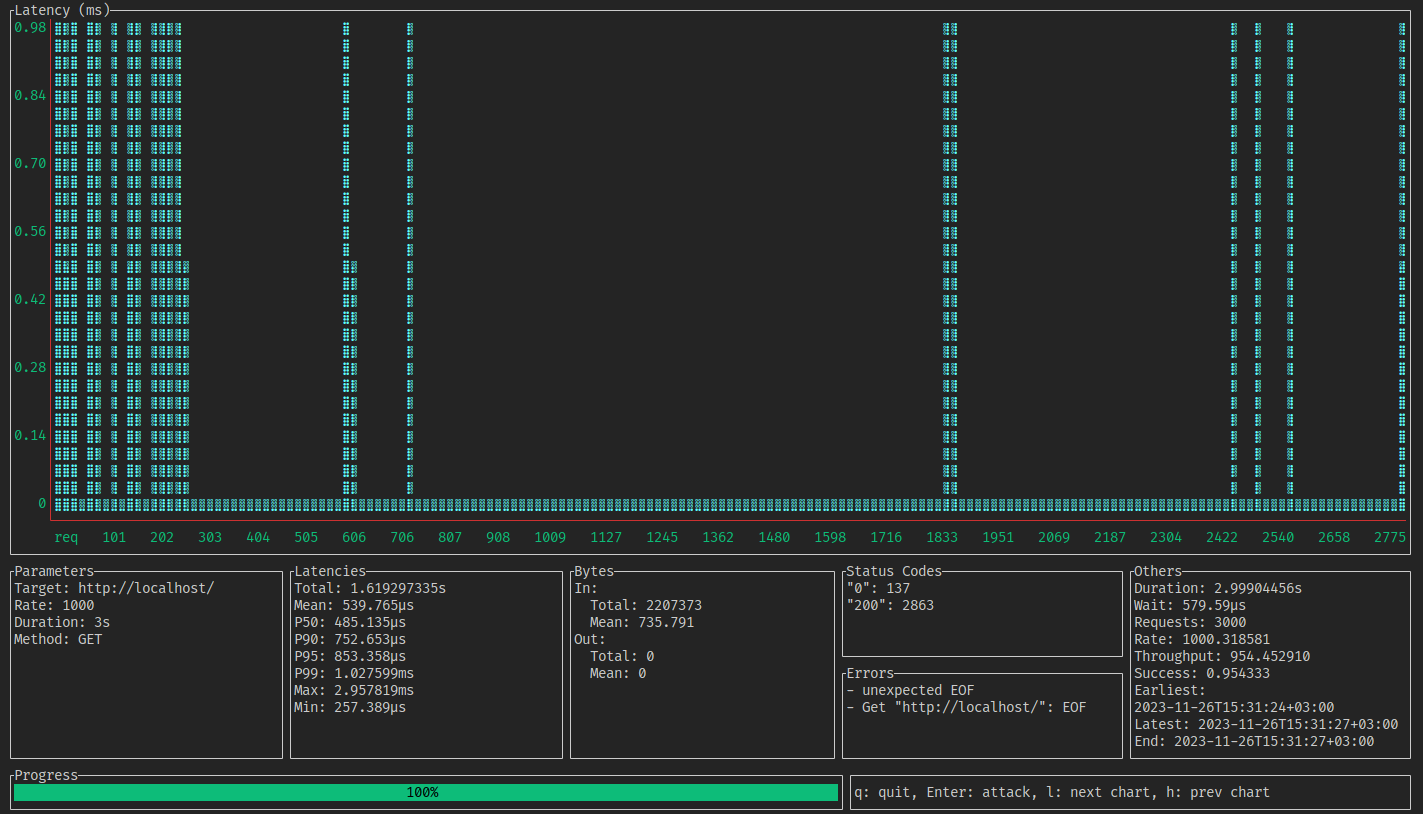
\includegraphics[width=0.95\linewidth]{inc/img/1000_select.png}
        \caption{Стресс тест 1000 запросов в секунду к index.html}
        \label{img:s1}
    \end{center}
\end{figure}


\begin{figure}[H]
    \begin{center}
        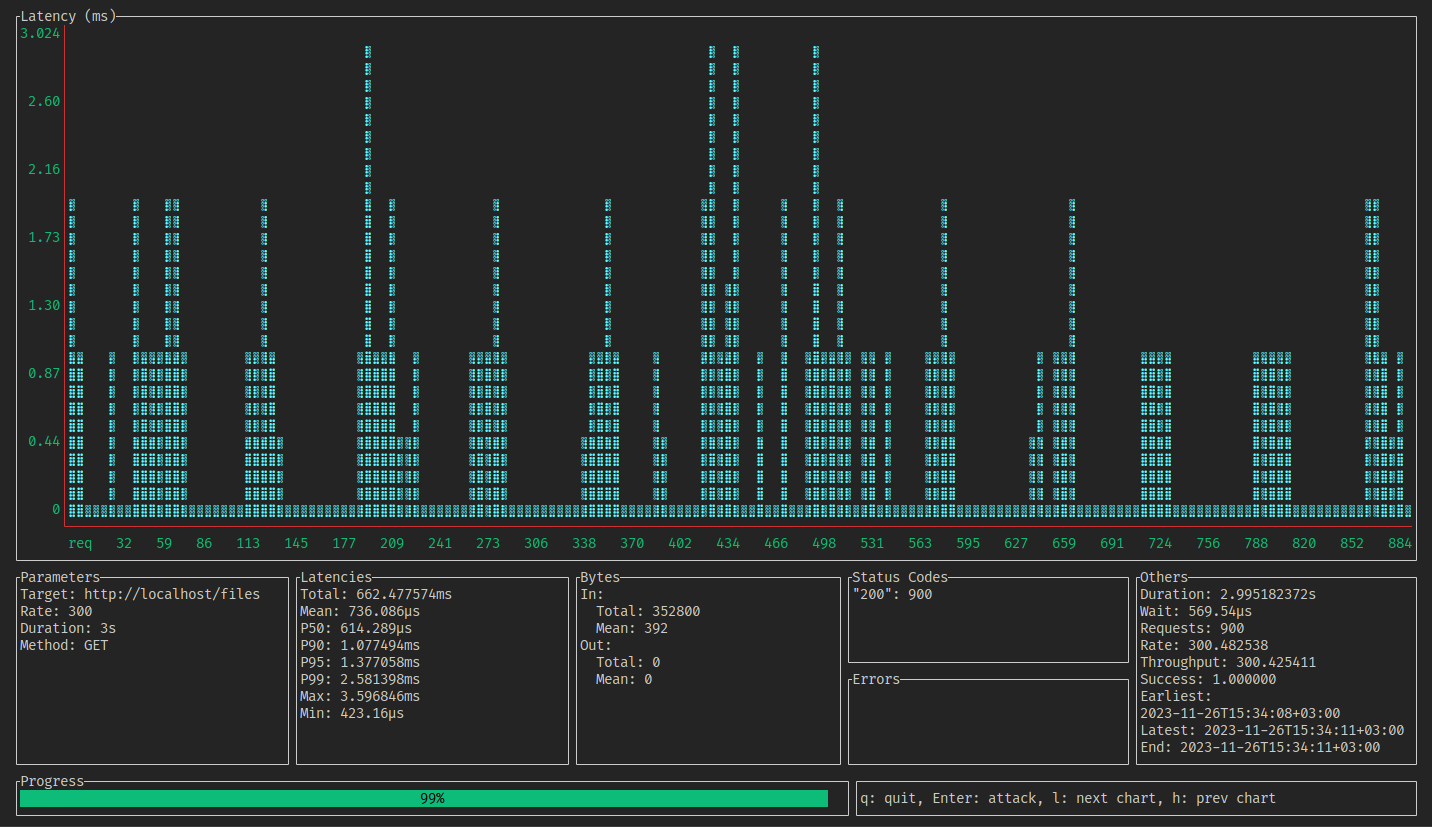
\includegraphics[width=0.95\linewidth]{inc/img/100_files.png}
        \caption{Стресс тест 100 запросов в секунду к директории с файлами}
        \label{img:s2}
    \end{center}
\end{figure}


\begin{figure}[H]
    \begin{center}
        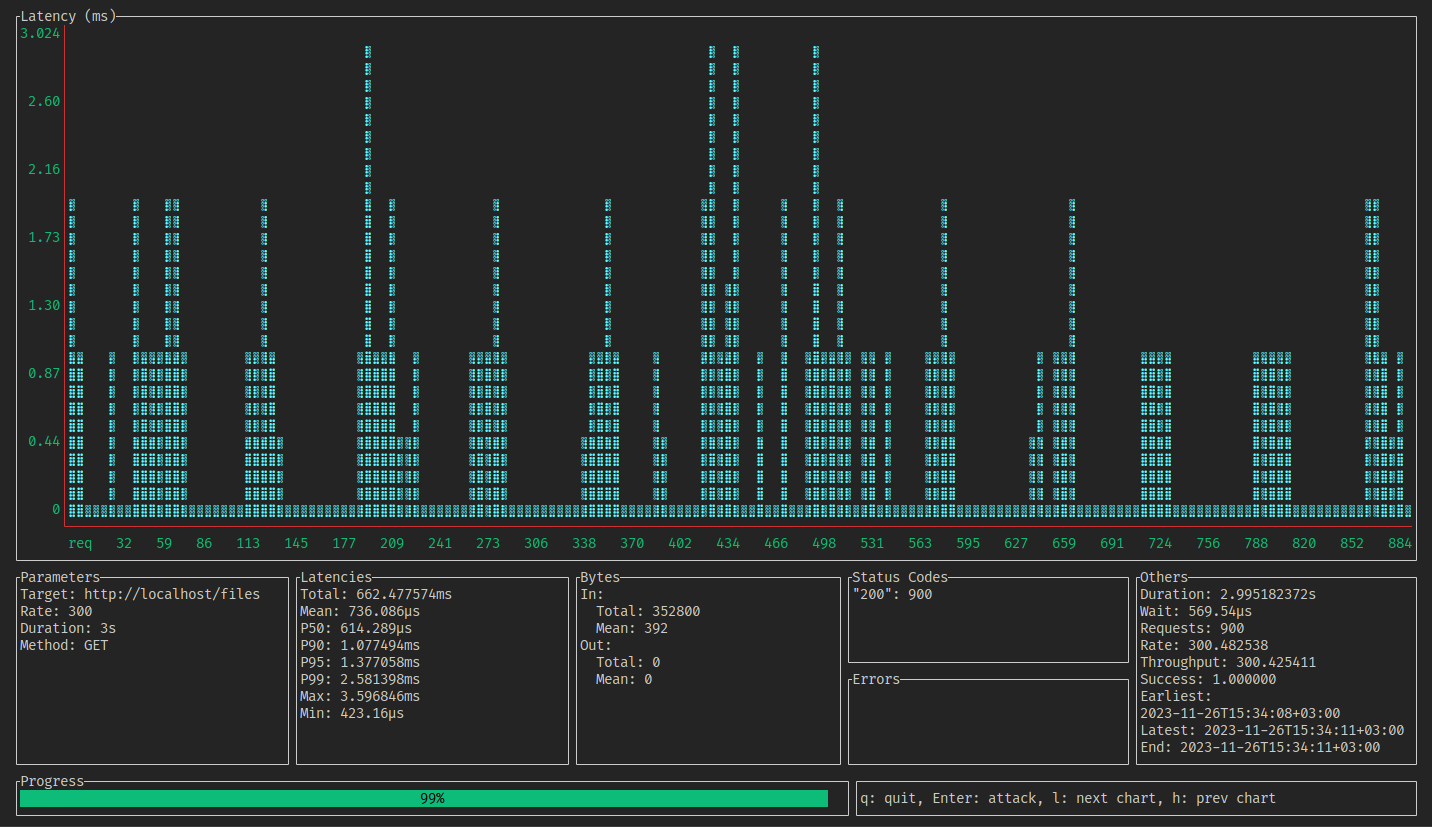
\includegraphics[width=0.95\linewidth]{inc/img/100_files.png}
        \caption{Стресс тест 100 запросов в секунду к изображению с котенком}
        \label{img:s3}
    \end{center}
\end{figure}

Если превысить 1000 запросов в секунду, возникают проблемы с файловыми дескрипторами select, и лучше использовать epoll, тоже реализованный в рамках курсовой.


\subsection{Сравнение с nginx}

На рисунке \ref{img:nginx} показано нагрузочное тестирование веб-сервера nginx. Он выдерживает куда большие нагрузки по сравнению с реализованным (50к запросов в секунду, в 100 раз больше). Это связано с большой кодовой базой и использованием select против poll.

\begin{figure}[H]
    \begin{center}
        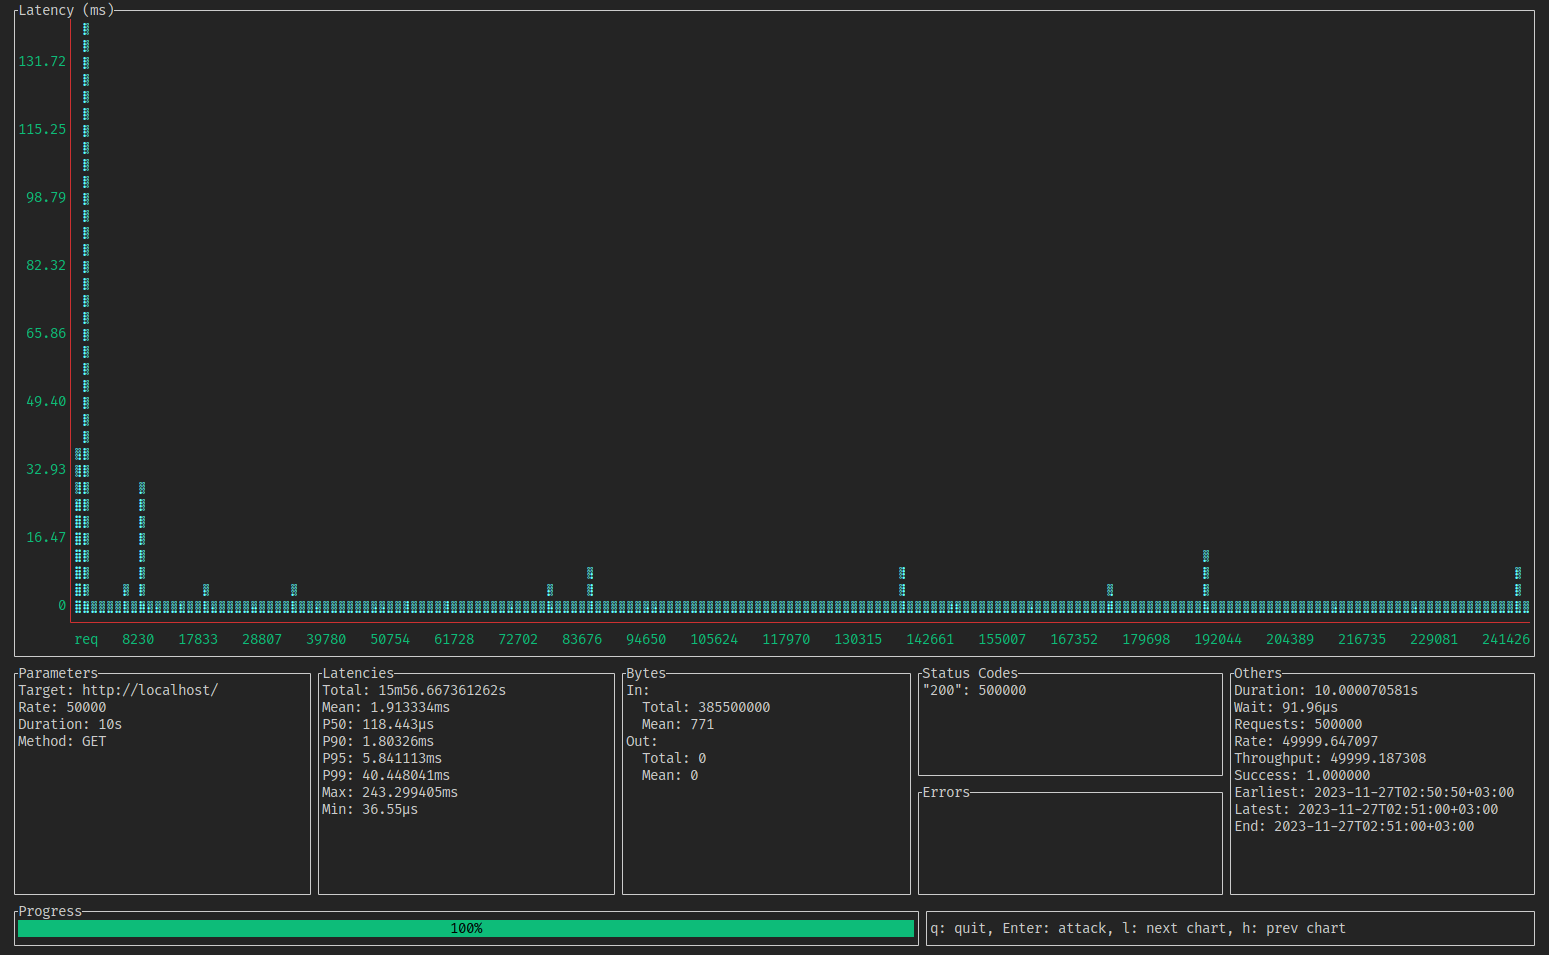
\includegraphics[width=0.95\linewidth]{inc/img/nginx.png}
        \caption{Стресс тест сервера nginx}
        \label{img:nginx}
    \end{center}
\end{figure}


\subsection{Вывод}
Проведено исследование стресс тестирование разработанного приложения и nginx, в ходе которого выявлено, что nginx работает лучше.